\newcommand{\rarrow}{\rightarrow}
\newcommand{\larrow}{\leftarrow}
\newcommand{\unif}{\sim}
\def\prop#1#2#3{\noindent\\$\begin{array}{l} \{#1\} \\ #2 \\ \{#3\} \\ \end{array}$\\\\}

\chapter{Modelação do Problema} \label{chap modprob}


\section{Modelação Informal}\label{sec modinf}
Com o diagrama da arquitectura do sistema, figura~\ref{fig diaact},pretende-se mostrar as várias entidades que podem aceder ao sistema, assim como as várias
actividades que cada uma pode realizar e tarefas para o sistema processar.
Também é realçada a ideia de que alguns dos recursos do sistema só estão dispóniveis ao utilizador depois 
de passar por outros passos, ou seja, o diagrama dá a entender a ordem pelas quais o utilizador e o sistema podem/devem executar as tarefas.\\

\begin{figure}[htbp]
\begin{center}
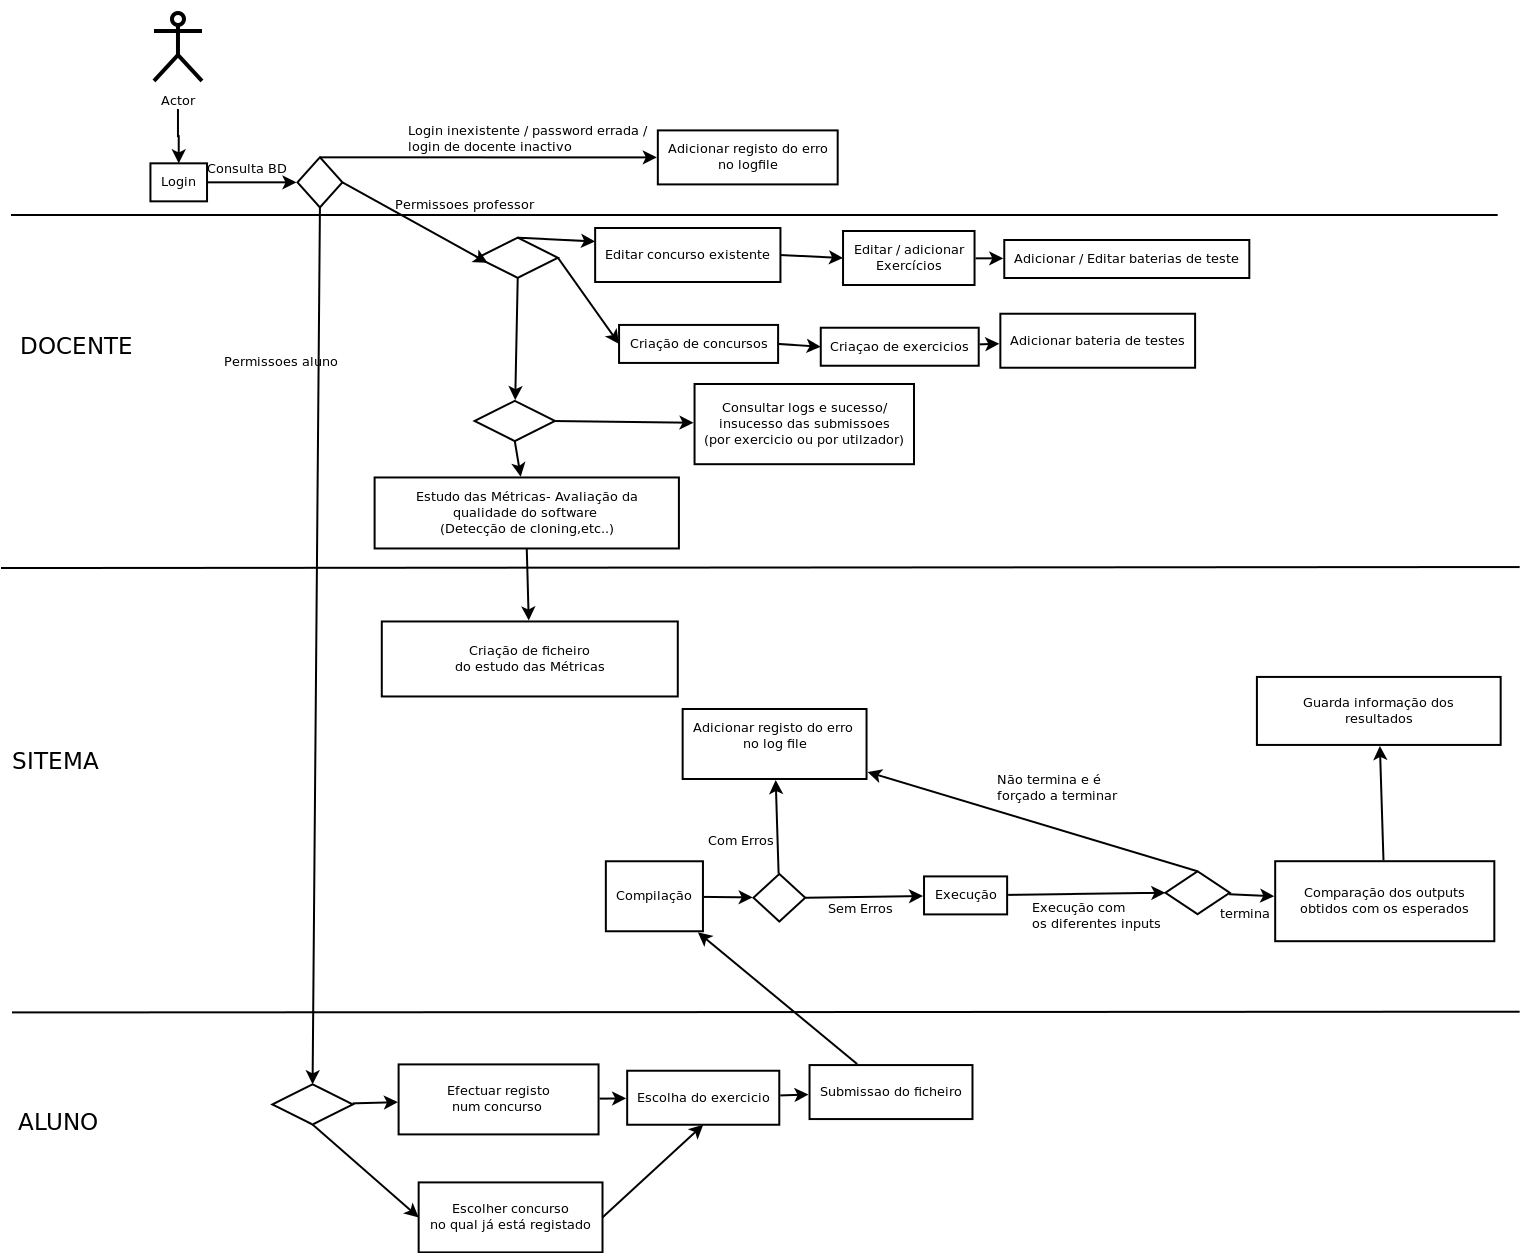
\includegraphics[width=0.9\textwidth]{Images/EL-PI}
\caption{Arquitectura do sistema}\label{fig diaact}
\end{center}
\end{figure}

Para começar, como temos duas entidades diferentes que podem aceder ao sistema (o docente e o aluno/concorrente), 
dividiu-se o diagrama em duas partes distintas (uma para cada entidade referida), de modo a facilitar a leitura.\\

Em ambos os casos, o login é a primeira actividade que pode ser realizada.
Se o login não foi efectuado com sucesso, é adicionado no log file uma entrada com a descrição do erro.
No caso de o login ser efectuado com sucesso, consoante as permissões do utilizador em questão, tem diferentes opções ao seu dispôr.\\

No caso do login pertencer a um docente, este terá acesso aos dados de cada um dos grupos, podendo verificar os resultados que estes 
obtiveram na resolução das questões do(s) concurso(s), assim como ao ficheiro que contém a análise das métricas dos vários programas submetidos 
pelos mesmos.
Poderá também criar novos concursos e os seus respectivos exercícios, assim como adicionar baterias de testes para os novos exercícios, 
ou para exercícios já existentes.\\

No caso do login pertencer a um aluno/concorrente, o utilizador terá a opção de se registar num concurso ou de seleccionar um no qual já 
esteja registado.
Já depois de seleccionar o concurso, pode ainda escolher o exercício que pretende submeter.
Depois de submeter o código fonte do programa correspondente ao exercício escolhido, e já sem a interacção do utilizador, 
o sistema compilará e tentará executar os diferentes inputs da bateria de testes do exercício, e compararar os resultados obtidos com os esperados.
No fim de cada um destes procedimentos, serão guardados os resultados / erros.
Para terminar, será feito um estudo das métricas do ficheiro submetido, tendo como resultado a criação um ficheiro com os dados relativos a essa avaliação.\\

\section{Modelação Formal}\label{sec modfor}

Afim de haver algum rigor na definição do sistema decidiu-se fazer um modelo mais formal do ponto de vista dos dados e das funcionalidades que o sistema apresenta.
A ideia desta modelação é ainda ser um modelo formal da especificação atrás descrita. Para isso utilizou-se uma notação orientada aos contratos (design by contract),
com a riqueza que as pré e pós condições de funções nos oferecem.\\

Assim sendo, temos descritos os contratos da seguinte forma:
$$\noindent\begin{array}{c} \{P\} \\ C \\ \{R\} \\ \end{array}$$
em que $P$ define uma pré condição, $C$ uma assinatura de uma função e $R$ uma pós condição.
De notar que tanto a pré como a pós condição teem de ser elementos booleanos e devem-se referir à assinatura da função. Assim sendo estamos a definir que apenas o contrato $C$
é válido se a sua pré e pós condições devolverem $true$. A pré e pós condição podem ser vazias.\\

Neste sistema que difinimos a assinatura $C$ da função pode ter uma particularidade, que é a instânciação de um elemento que pertença a um determinado tipo.
Ou seja, pode-se dizer $$soma :: a \unif Int \rarrow b \unif Int \rarrow Int$$ para expressar que a função $soma$ recebe dois parametros $a$ e $b$ que são inteiros e devolve
um elemento do tipo inteiro.\\

Decidimos, por motivos de facilidade de leitura e afim de evitar a complexidade formal, não especificar o estado interno do sistema, como por exemplo o estado do Apache,
da base de dados entre outros componentes do sistema. Achamos que especificar isso não iria trazer nada de interessante ao que pretendemos mostrar aqui.
Assim, neste modelo formal apenas se vê de forma clara, os contratos que queremos que o nosso sitema tenha.\\

Começamos então por definir o contrato da função $login$ que permite a um determinado utilizador entrar no sistema. Este contrato estipula que recebendo um par
$Username \times Hash$ e um $SessionID$ devolve ou um $Error$ ou um novo $SessionID$ que associa o utilizador à sua sessão no sistema. Afim de haver provacidade
sobre os dados criticos do utilizador, como a password, decidimos apenas receber do lado do servidor a $Hash$ respectiva da sua palavra-passe, sendo esta hash
gerada do lado do cliente. Esta técnica não tem nada de novo, mas por incrível que pareça ainda há sistemas online que não usam este tipo de mecanismos.\\

\prop
{existsInDatabase(u)}
{login :: u \unif Username \times Hash \rarrow SessionID \rarrow Error + SessionID}
{ }

Aprenta-se de seguida o modelo de dados formal que o sistema usa. Consideramos que um $Exercicio$ tem um $Enunciado$ e um dicionário a relacionar $Input's$ com $Output's$,
um concurso tem um nome, um tipo e um conjunto de exercicios.\\

$\begin{array}{l}
data~Dict~a~b = (a \times b)^{*} \\
data~Exercicio = Exercicio~Enunciado~(Dict~Input~Output) \\
data~Contest =  Contest~Nome~Tipo~Exercicio^{*}
\end{array}$\\

Para criar um novo concurso, temos de assegurar que o utilizador que requisita este serviço é um professor, visto não nos interessar que alunos criem concursos.
Temos ainda de assegurar que o concurso que se vai criar tem no minimo um exercicio.\\

\prop
{ existeSession(s)  \wedge isProf(s) \wedge (notEmpty \circ getExercice)~c}
{createContest :: s \unif SessionID \rarrow c \unif Contest \rarrow 1}
{ (notEmpty \circ getDict)~c }

Para criar um novo exercicio, o utilizador tem de ser um professor e o exercicio em questão não pode ser repetido no sistema. Decidiu-se assim para evitar redundância
na informação que se tem armazenada.

\prop
{ existeSession(s)  \wedge isProf(s) \wedge (not \circ exist) (Exercicio e d)}
{createExercice :: s\unif SessionID \rarrow e \unif Enunciado \rarrow d \unif (Dict a b) \rarrow 1}
{ exerciceCreated(Exercicio e d) }

Pode-se ainda consultar os logs de um concurso especifico. Aqui apresentamos como argumento toda o concurso - $Contest$ para apenas evitar a definição evidente
de identificadores. É claro que a implementação desta acção, irá receber como parametro o identificador do concurso, como em outros parametros deste modelo formal.

\prop 
{ existeSession(s) \wedge isProf(s) \wedge contestIsClosed(c) }
{consultarLogsContest :: s \unif SessionID \rarrow c \unif Contest \rarrow LogsContest}
{}

De seguida mostra-se a especificação de efectuar um registo no concurso, queremos apenas que o concurso não esteja cheio.

\prop
{ existSession(s) \wedge contestNotFull(c)}
{registerOnContest :: s \unif SessionID \rarrow c\unif Contest \rarrow Credenciais}
{ }

Pode-se ainda sumbmeter um exercicio, o que implica que esta acção tenha como consequência devolver um relatório com os resultados interessantes para monstrar
ao participante de um concurso.

\prop
{ existeSession(s) \wedge exerciceExist(e) }
{ submitExercicio :: s \unif SessionID \rarrow e \unif Exercicio \rarrow res \unif Resolucao \rarrow rep \unif Report}
{ rep = geraReport s e res }

\subsubsection{Modelação de acções de selecção}
Temos acções do nosso sistema que envolvem a selecção de items nos forms ou então métodos que geram efeitos secundários, assim decidimos explicar aqui esse conjunto de
contractos. Estes métodos são interessantes de modelar porque, assim fica mais claro ver os parametros que recebemos para os concretizar.\\

Temos então a acção de escolha de um exercicio numa panoplia de exercicios disponiveis no concurso que o utilizador está actualmente inscrito e a participar.\\
Relembramos que o uso do tipo $1$ significa o tipo unitário, ou seja, queremos denotar que do ponto de vista formal esta operação não devolve nada, apenas altera o sistema.
Sistema esse que no inicio explicamos que por motivos de complexidade não tinha interesse expecificar formalmente.

\prop
{ existeSession(s) \wedge exerciceExist(e) }
{escolheExercicio :: s \unif SessionID \rarrow e \unif Exercicio \rarrow 1}
{ }

Temos ainda a escolha do concurso para um grupo que está já registado.

\prop
{ existSession(s) \wedge existContest(c) \wedge userRegistadoNoContest(s,c) }
{escolheConcursoJaRegistado :: s \unif SessionID \rarrow c \unif Contest \rarrow 1}
{ }

Mostramos de seguida o contracto da função que gera um relatório ao concorrente.

\prop
{ }
{geraReport :: e \unif Exercicio \rarrow res \unif Resolucao \rarrow Report}
{ }

A titulo de exemplo, da potencialidade deste tipo de modelação, servimo-nos agora da linguagem do Haskell para especificar a definição desta operação em maior detalhe.
Temos então as seguintes definições:

\begin{eqnarray*}
geraReportBugCompile :: Exercicio \rarrow Error \rarrow Report\\
geraReportBugCompare :: Exercicio \rarrow Errado \rarrow Report\\
geraReportNoBug :: Exercicio \rarrow Resolucao \rarrow Report\\
\\
execute :: Program \rarrow Exercicio \rarrow ResolucaoProposta\\
\end{eqnarray*}

Temos ainda que $ResolucaoProposta$ é a resolução submetida pelos concorrentes e aprenstenta o seguinte tipo:

$\begin{array}{l}
data~ResolucaoProposta = Dict~Input~Output
\end{array}$\\

Temos ainda a função que recebe uma resolução como input e devolve ora um programa pronto já compilado, ora um erro no caso de surgir algum problema na compilação.

\prop
{ }
{compile :: Resolucao \rarrow Error + Program}
{ }

E ainda uma função de comparação que recebe uma resolução e um exercicio e devolve se o Output pretendido é o mesmo que o que o programa submetido origina.

\prop
{ length(Exercicio)==length(ResolucaoProposta)}
{compare :: Exercicio \rarrow ResolucaoProposta \rarrow Certo + Errado}
{ }

\begin{lstlisting}[language=HaskellUlisses]
geraReport :: Exercicio -> Resolucao -> Report
geraReport exer res = do
	case compile res of
		(Left error) -> geraReportBugCompile error res
		(Right p) ->
			let resProps = execute p exer
			in case (compare exer resProps) of
				(Left certo) -> geraReportNoBug e res
				(Right errado) -> geraReportBugCompare errado res
\end{lstlisting}

Se quisessemos este código de um ponto de vista de composição de funções a sua conversão poderia ser fácilmente atingida pelas seguintes definições:

\begin{lstlisting}[language=HaskellUlisses]
geraReport exer res =
	compile res >>= \p -> compare exer (execute p exer)
		>>= \c -> geraReportNoBug exer res
\end{lstlisting}

%geraReport e res = compile res >>= \p \rarrow compare(e (execute p e)) >>= pageCerto)

Temos ainda o contrato da função que gera o relatório final baseando-se na participação de uma equipa num determinado concurso.

\prop
{ existSession(s) \wedge existContest(c) \wedge }
{geraFinalReport :: s \unif SessionID \rarrow c \unif Contest \rarrow Dict Exercicio Resolucao \rarrow Report}
{ }

\section{Modelo de Dados}\label{sec modedados}

Definiu-se que existirão três tipos de utilizadores: o administrador, o docente e o grupo.\\

\begin{itemize}
  \item Administrador - é a entidade com mais poder no sistema. É o único que pode criar contas do tipo docente. É caracterizado por:
    \begin{itemize}
      \item Nome de utilizador;
      \item Nome completo;
      \item Password
      \item e-Mail
    \end{itemize}
  \item Docente - entidade que tem permissões para criar concursos, exercícios, aceder aos resultados das submissões, (...). 
Os seus atributos coincidem com os do Administrador.
  \item Grupo - entidade que pode registar-se em concursos e submeter tentativas para os seus diferentes enunciados.
\end{itemize}

Decidiu-se que o sistema terá a noção de grupo, e um grupo não é mais do que um conjunto de concorrentes. No entanto,
o grupo é que possui as credenciais para entrar no sistema (nome de utilizador e password). 
Além disso também tem um nome pelo qual é identificado, um e-mail que será usado no caso de haver necessidade de se entrar em contacto
com o grupo, e um conjunto de .\\

Achamos importante incluir a informação de cada concorrente no grupo para, se possível, automatizar várias tarefas tais como lançamento de notas.
Cada concorrente é caracterizado pelo seu nome completo, número de aluno (se for o caso), e e-mail.\\

\begin{figure}[htbp]
\begin{center}
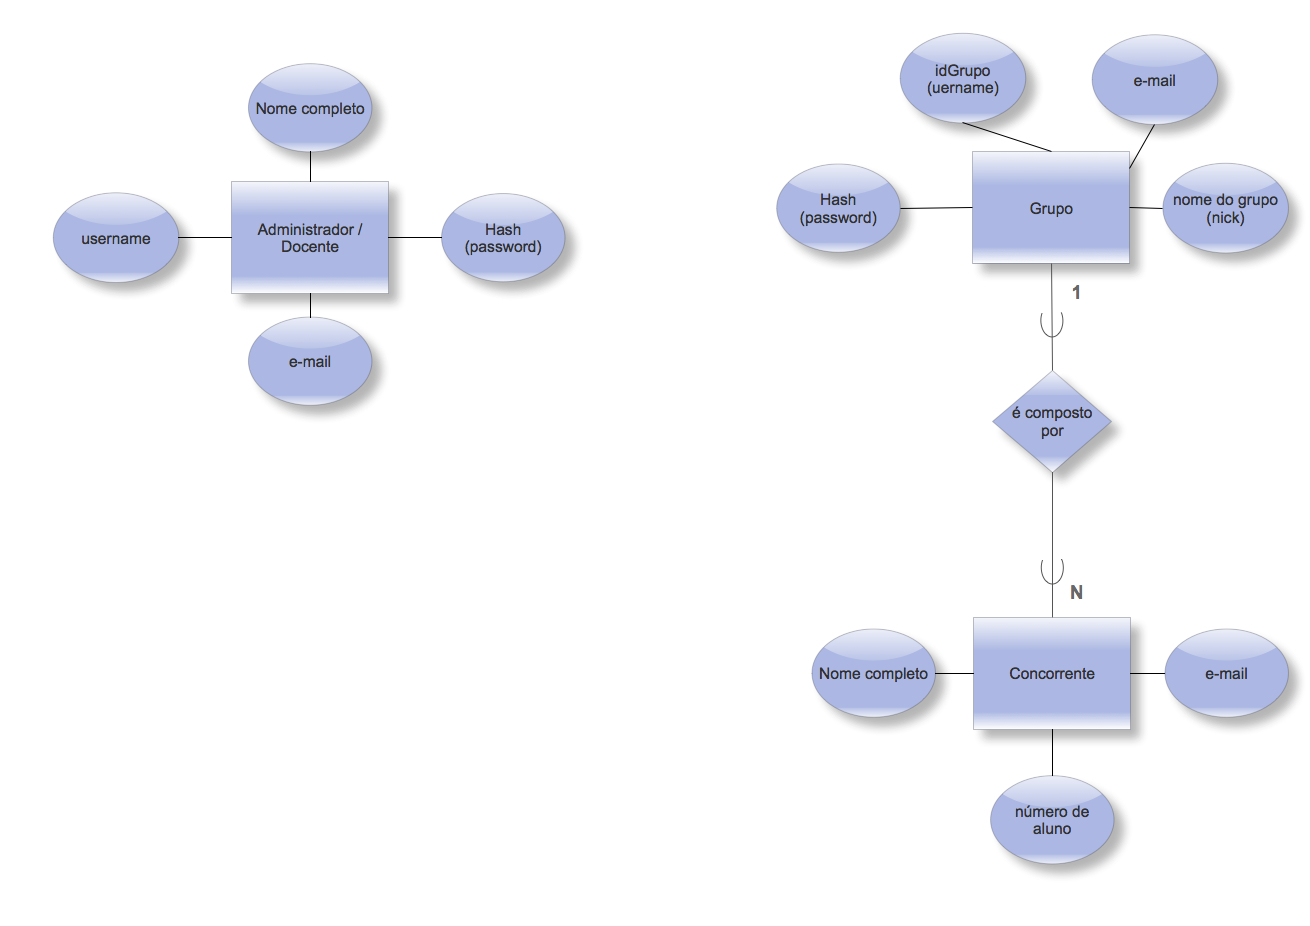
\includegraphics[width=0.9\textwidth]{Images/grupo-docente}
\caption{Modelo de dados - Grupo e Docente/Admin}\label{fig modedados-grupo-doc}
\end{center}
\end{figure}


Para finalizar vamos explicar em que consistem os concursos, enunciados e tentativas.

Um concurso, resumidamente, é um agregado de enunciados. 
Tem outras propriedades tais como um título, data de inicio e data de fim (período em que o concurso está disponível para que os grupos se registem), 
chave de acesso (necessária para o registo dos grupos), duração do concurso (tempo que o grupo tem para resolver os exercícios do concurso, 
a partir do momento que dá inicio à prova), e por fim, regras de classificação.\\
\\
Um enunciado é um exercício que o concorrente tenta solucionar. Como seria de esperar, cada exercício pode ter uma cotação diferente, 
logo o peso do enunciado é guardado no mesmo. 
Para cada enunciado existe também um conjunto de inputs e outputs, que servirão para verificar se o programa submetido está correcto. 
Contém ainda uma descrição do problema que o concorrente deve resolver, assim como uma função de avaliação, função esta que define como
 se verifica se o output obtido está de acordo com o esperado.\\
\\
Uma tentativa é a informação que é gerada pelo sistema, para cada vez que o grupo submete um ficheiro.\\
Além de conter dados sobre o concurso, enunciado e grupo a que pertence, a tentativa também contém o caminho para o código fonte do programa
submetido, data e hora da tentativa, dados referentes à compilação e um dicionário com os inputs esperados e os outputs gerados pelo programa
submetido.
\begin{figure}[htbp]
\begin{center}
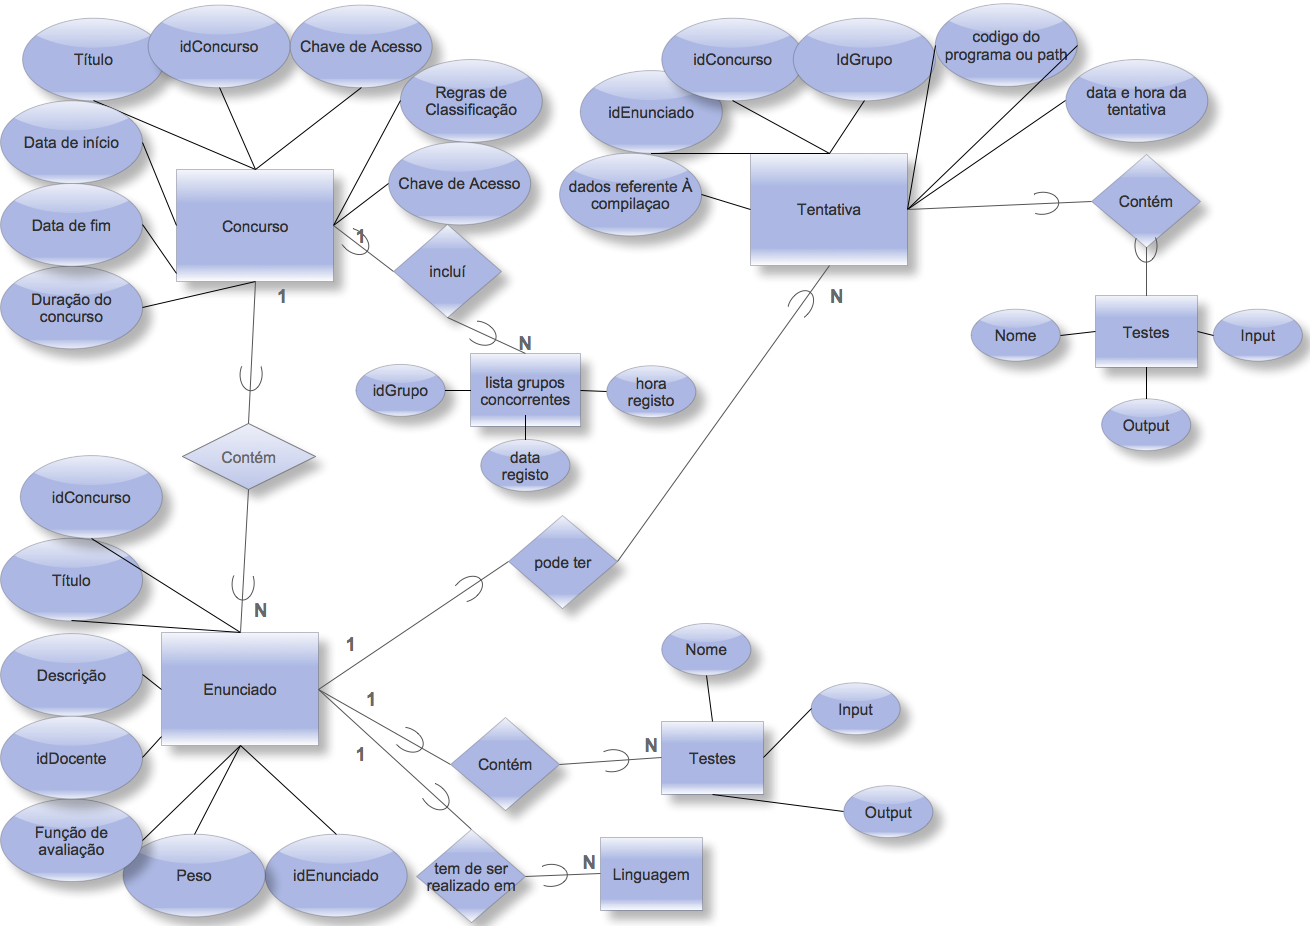
\includegraphics[width=0.9\textwidth]{Images/concurso-enunciado}
\caption{Modelo de dados - Concurso, tentativa e enunciado}\label{fig modedados-conc-enunc}
\end{center}
\end{figure}

\section{Importação de dados}\label{sec xml}

Uma das funcionalidades requeridas ao nosso sistema é a importação de enunciados e tentativas no formato xml.
Esta funcionalidade será bastante útil para demonstrar e testar o sistema, sem que se tenha de criar manualmente os enunciados
 usando a interface gráfica, ou se tenha que submeter ficheiros com código fonte, de modo a serem geradas tentativas.
Os campos presentes no xml de cada uma das entidades, \textit{enunciado} e \textit{tentativa}, são praticamente os mesmos 
que estão descritos no modelo de dados das respectivas entidades.\\
\\
No xml do enunciado, não há nada muito relevante a acrescentar, além de que não contém um id para o enunciado, pois este será gerada 
automaticamente pelo sistema. Passamos agora a apresentar um exemplo do mesmo.
\\
\lstinputlisting{resources/enunciado.xml}


Quanto ao xml para a \textit{tentativa} há que realçar o facto de que o código fonte do programa vai dentro de uma tag xml.  Além da tag xml, o código fonte
terá de ir cercado de uma secção CDATA. Isto acontece para que o que o código fonte não seja processado com o restante xml que o contém.\\
\\

\lstinputlisting{resources/tentativa.xml}


Para que todos os dados contidos nos ficheiros xml possam ser facilmente validados, foram criados dois \textit{XML schema}.
Neste schema definimos quais as tags que devem existir em cada xml, o tipo de dados e até a gama de valores que serão contido por cada tag e
 a multiplicidade das tags .\\

Nesta fase inicial do projecto ainda não foram sempre especificados  os tipos de dados que serão contidos por cada tag.\\
No entanto, para alguns dos casos em que tal aconteceu apresentaremos alguns exemplos e explicações.\\
\\
No xsd referente ao \textit{enunciado} encontramos o elemento \textit{Peso}, que é um exemplo de uma tag que contém restrições.
O \textit{Peso} terá de ser um inteiro e terá um valor entre 0 e 100.

\begin{lstlisting}
<ed:element name="Peso" default="25">
  <ed:simpleType>
    <ed:restriction base="ed:integer">
      <ed:minInclusive value="0"/>
      <ed:maxInclusive value="100"/>
    </ed:restriction>
  </ed:simpleType>
</ed:element>
\end{lstlisting}
Já o elemento \textit{Linguagem} é também restringido, mas de uma forma ligeiramente diferente. A \textit{Linguagem} será uma string, mas
apenas poderá tomar um dos valores enumerados no xsd.\\

\begin{lstlisting}
<ed:element name="Linguagem" maxOccurs="unbounded">
    <ed:simpleType>
	<ed:restriction base="ed:string">
	    <ed:enumeration value="C"/>
	    <ed:enumeration value="Java"/>
	    <ed:enumeration value="Haskell"/>
	</ed:restriction>
    </ed:simpleType>
</ed:element>
\end{lstlisting}


No xsd para a \textit{tentativa} podemos evidenciar a multiplicidade das tags, ou seja, quantas vezes algumas delas se podem repetir.
Na \textit{tentativa}, existe um \textit{Dict}, que contém uma ou mais tags \textit{Teste}.
Para definirmos que possam existir mais de que uma tag \textit{Teste} dentro de \textit{Dict}, adicionamos o atributo \textit{maxOccurs},
na entidade \textit{Teste}, com o valor \textit{``unbounded''}. O valor mínimo não é necessário definir, porque é um por default.
\begin{lstlisting}
<tt:element name="Dict">
    <tt:complexType>
	<tt:sequence>
	    <tt:element name="Teste" maxOccurs="unbounded">
		<tt:complexType>
		    <tt:sequence>
			<tt:element name="Nome" type="tt:string"/>
			<tt:element name="Input" type="tt:string"/>
			<tt:element name="Output" type="tt:string"/>
		    </tt:sequence>
		</tt:complexType>
	    </tt:element>
	</tt:sequence>
    </tt:complexType>
</tt:element>
\end{lstlisting}

Para dar uma ideia mais geral sobre ambos os \textit{xml schema} criados, em vez de apresentarmos aqui ambos os ficheiros integralmente,
vamos antes expor os diagramas que o programa \textit{oxygen} constrói e coloca ao nosso dispor, pois pensamos que torna o entendimento do
schema muito mais simples.\\
\newpage
Desta forma aqui ficam os diagramas para o enunciado e para a tentativa:\\
 
\begin{figure}[htbp]
\begin{center}
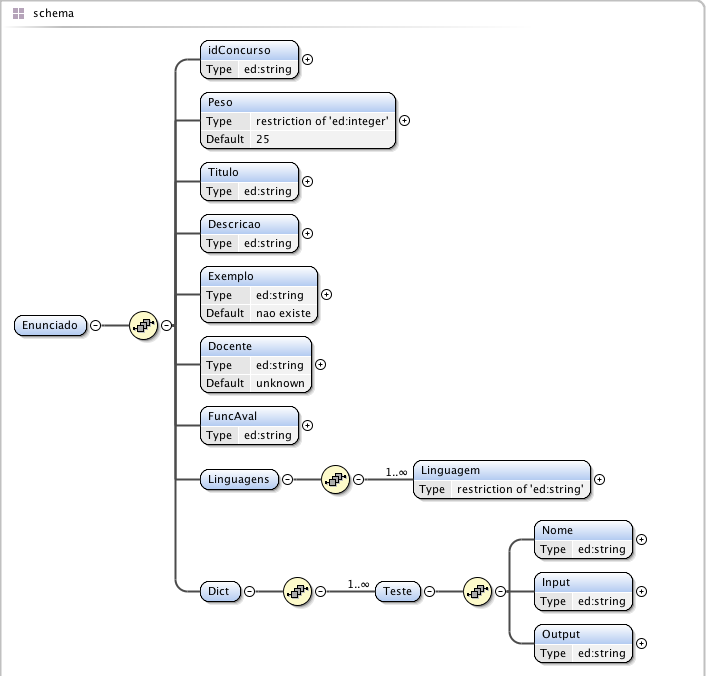
\includegraphics[width=0.9\textwidth]{Images/enunciado_schema}
\caption{diagrama do schema para o enunciado}\label{fig xsd enunciado}
\end{center}
\end{figure}

\begin{figure}[htbp]
\begin{center}
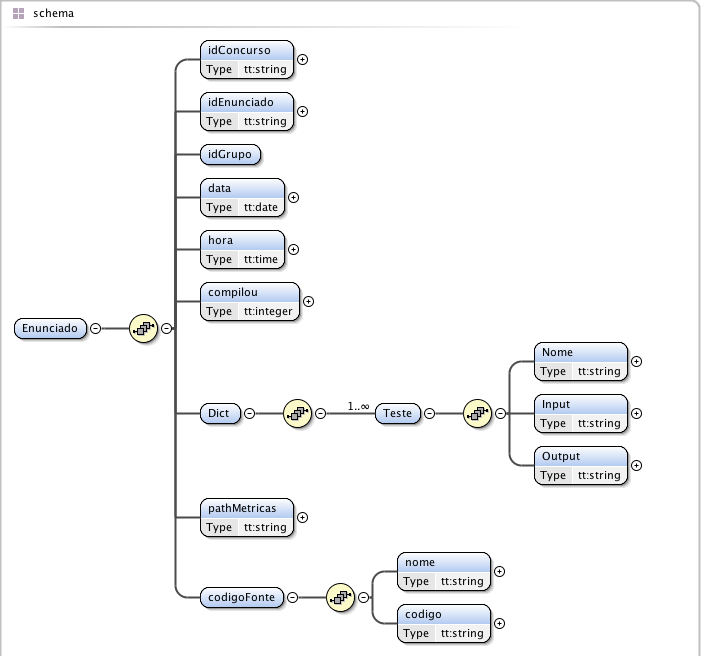
\includegraphics[width=0.9\textwidth]{Images/tentativa_schema}
\caption{diagrama do schema para a tentativa}\label{fig xsd tentativa}
\end{center}
\end{figure}
